\documentclass{article}
\usepackage[utf8]{inputenc}
\usepackage[english]{babel}

\usepackage{graphicx}
\usepackage[margin=2.5cm]{geometry}
\usepackage{amssymb}
\usepackage{amsmath}
\setcounter{MaxMatrixCols}{20}%%aumentar el numero de columnas en una matriz
\usepackage{arydshln}%% dot line in matrix
\usepackage{mathtools}%% dot line in matrix
\usepackage{arydshln}
\usepackage{hyperref}
\usepackage{float}

\usepackage{titlesec}

\usepackage{comment}

\usepackage{biblatex}
\addbibresource{refrence.bib}


\title{Path Filling Points}
\author{Fernando Pujaico Rivera}
\begin{document}
\maketitle 

\tableofcontents




%%%%%%%%%%%%%%%%%%%%%%%%%%%%%%%%%%%%%%%%%%%%%%%%%%%%%%%%%%%%%%%%%%%%%%%%%%%%%
%%%%%%%%%%%%%%%%%%%%%%%%%%%%%%%%%%%%%%%%%%%%%%%%%%%%%%%%%%%%%%%%%%%%%%%%%%%%%
\section{3D parametric linear spline }
A 3D parametric linear spline is a parametric function defined piecewise by parametric polynomials in $\mathbb{R}^{3}$ space.
The Fig. \ref{fig:3DLinearSplinePoly} shows the polynomials $\mathbf{\hat{p}}^{(n)}(t)$ with parameter $t$ 
close to the n-th position.
\begin{figure}[H]
    \centering
    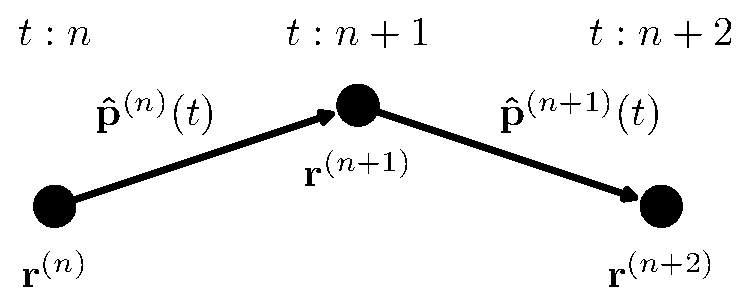
\includegraphics[width=0.35\textwidth]{boveda/Diagrama0.eps}
    \caption{Polynomials in the n-th position of linear spline}
    \label{fig:3DLinearSplinePoly}
\end{figure}

Given a set of $N$ points $\mathbf{r}^{(n)}\in\mathbb{R}^{3}$, $\forall$ $0\leq n \leq N-1$, 
we can generate a linear spline with $N-2$ polynomials $\mathbf{\hat{p}}^{(n)}(t)$, $\forall$ $0\leq n \leq N-2$, 
according to Fig. \ref{fig:3DLinearSplinePoly}.
So that, it is fulfilled that 

\begin{equation}
\mathbf{\hat{p}}^{(n)}(t)=
\begin{bmatrix}
\hat{x}^{(n)}(t) & \hat{y}^{(n)}(t) & \hat{z}^{(n)}(t),
\end{bmatrix}^{T}
\end{equation}
where
\begin{equation}
\hat{x}^{(n)}(t)=\hat{a}_{x}^{(n)}+\hat{b}_{x}^{(n)}(t-n),
\end{equation}
\begin{equation}
\hat{y}^{(n)}(t)=\hat{a}_{y}^{(n)}+\hat{b}_{y}^{(n)}(t-n),
\end{equation}
\begin{equation}
\hat{z}^{(n)}(t)=\hat{a}_{z}^{(n)}+\hat{b}_{z}^{(n)}(t-n).
\end{equation}



%%%%%%%%%%%%%%%%%%%%%%%%%%%%%%%%%%%%%%%%%%%%%%%%%%%%%%%%%%%%%%%%%%%%%%%%%%%%%
\subsection{Matricial form of polynomials $\mathbf{\hat{p}}^{(n)}(t)$}
For all values $0\leq n \leq N-2$, we know that
\begin{equation}
\mathbf{\hat{w}}^{(n)}=
\left[
\begin{array}{cc:cc:cc}
\hat{a}_{x}^{(n)} & \hat{b}_{x}^{(n)} & 
\hat{a}_{y}^{(n)} & \hat{b}_{y}^{(n)} & 
\hat{a}_{z}^{(n)} & \hat{b}_{z}^{(n)} 
\end{array}
\right]^{T},
\end{equation}
\small
\begin{equation}\label{eq:hatAnt}
\mathbf{\hat{A}}^{(n)}(t)=
\left[
\begin{array}{cc:cc:cc}
1 & (t-n) &
0 & 0     &
0 & 0     \\
0 & 0     &
1 & (t-n) &
0 & 0     \\
0 & 0     &
0 & 0     &
1 & (t-n) 
\end{array}
\right],
\end{equation}
\normalsize

\begin{equation}\label{eq:hatprimeder0}
\mathbf{\hat{p}}^{(n)}(t)=
\mathbf{\hat{A}}^{(n)}(t) \mathbf{\hat{w}}^{(n)}.
\end{equation}

Additionally, we can define

\begin{equation}
\mathbf{\hat{w}}
\equiv
\begin{bmatrix}
\mathbf{\hat{w}}^{(0)}\\
\mathbf{\hat{w}}^{(1)}\\
%\mathbf{\hat{w}}^{(2)}\\
\vdots\\
\mathbf{\hat{w}}^{(N-2)}\\
\end{bmatrix}
\in \mathbb{R}^{6(N-1)}
\end{equation}


%%%%%%%%%%%%%%%%%%%%%%%%%%%%%%%%%%%%%%%%%%%%%%%%%%%%%%%%%%%%%%%%%%%%%%%%%%%%%
%%%%%%%%%%%%%%%%%%%%%%%%%%%%%%%%%%%%%%%%%%%%%%%%%%%%%%%%%%%%%%%%%%%%%%%%%%%%%
\subsection{Boundary conditions in 3D parametric linear spline}\label{sec:boundarylinear}

%%%%%%%%%%%%%%%%%%%%%%%%%%%%%%%%%%%%%%%%%%%%%%%%%%%%%%%%%%%%%%%%%%%%%%%%%%%%%
\subsubsection{Conditions in points}

Following the Fig. \ref{fig:3DLinearSplinePoly}, 
we can affirm that for $0 \leq n\leq N-2$,
so that
\begin{equation}\label{eq:hatcondition1}
\mathbf{\hat{p}}^{(n)}(n)=\mathbf{r}^{(n)}
\in \mathbb{R}^{3},
\end{equation}

\begin{equation}\label{eq:hatcondition2}
\mathbf{\hat{p}}^{(N-2)}(N-1)=\mathbf{r}^{(N-1)}
\in \mathbb{R}^{3},
\end{equation}

\textbf{Matricial form of the conditions in points:}

Using 
the Eq. \ref{eq:hatprimeder0} in 
the Eqs. \ref{eq:hatcondition1} and \ref{eq:hatcondition2},
we obtain for $0 \leq n\leq N-2$

\begin{equation}\label{eq:hatpointcond1}
\mathbf{\hat{A}}^{(n)}(n) \mathbf{\hat{w}}^{(n)}=\mathbf{r}^{(n)}
\in \mathbb{R}^{3},
\end{equation}

\begin{equation}\label{eq:hatpointcond2}
\mathbf{\hat{A}}^{(N-2)}(N-1) \mathbf{\hat{w}}^{(N-2)}=\mathbf{r}^{(N-1)}
\in \mathbb{R}^{3},
\end{equation}


where, using the Eq. \ref{eq:hatAnt}, we know that

\begin{equation}\label{eq:hatQ00}
\mathbf{\hat{A}}^{(n)}(n+1)=
\left[
\begin{array}{cc:cc:cc}
1 & 1 & 0 & 0 & 0 & 0 \\
0 & 0 & 1 & 1 & 0 & 0 \\
0 & 0 & 0 & 0 & 1 & 1 
\end{array}
\right]
\equiv \mathbf{\hat{Q}}^{(0,0)}\in \mathbb{R}^{3\times 6},
\end{equation}

\begin{equation}\label{eq:hatQ01}
\mathbf{\hat{A}}^{(n+1)}(n+1)
=
\mathbf{\hat{A}}^{(n)}(n)
=
\left[
\begin{array}{cc:cc:cc}
1 & 0 & 0 & 0 & 0 & 0 \\
0 & 0 & 1 & 0 & 0 & 0 \\
0 & 0 & 0 & 0 & 1 & 0 
\end{array}
\right]
\equiv \mathbf{\hat{Q}}^{(0,1)}\in \mathbb{R}^{3\times 6},
\end{equation}

Thus,
using the Eqs. \ref{eq:hatQ00} and \ref{eq:hatQ01} in 
the Eqs. \ref{eq:hatpointcond1} and \ref{eq:hatpointcond2}, $\forall 0 \leq n\leq N-2$.
We can write the Eqs. \ref{eq:hatcondition1} and \ref{eq:hatcondition2} as 

\begin{equation}
\mathbf{\hat{P}}
\mathbf{\hat{w}}
=\mathbf{r}\in \mathbb{R}^{3N}.
\end{equation}

Where

\begin{equation}
\mathbf{\hat{P}}
\equiv
\begin{bmatrix}
\mathbf{\hat{Q}}^{(0,1)} & \mathbf{0}         & \hdots & \mathbf{0} & \mathbf{0}         & \mathbf{0}\\
\mathbf{0}         & \mathbf{\hat{Q}}^{(0,1)} & \hdots & \mathbf{0} & \mathbf{0}         & \mathbf{0}\\
\vdots             & \vdots             & \vdots & \vdots     & \vdots             & \vdots    \\ 
\mathbf{0}         & \mathbf{0}         & \hdots & \mathbf{0} & \mathbf{\hat{Q}}^{(0,1)} & \mathbf{0}\\
\mathbf{0}         & \mathbf{0}         & \hdots & \mathbf{0} & \mathbf{0}         & \mathbf{\hat{Q}}^{(0,1)}\\
\mathbf{0}         & \mathbf{0}         & \hdots & \mathbf{0} & \mathbf{0}         & \mathbf{\hat{Q}}^{(0,0)}
\end{bmatrix}
\in \mathbb{R}^{3N\times 6(N-1)}
\end{equation}

and 

\begin{equation}
\mathbf{r}
\equiv
\begin{bmatrix}
\mathbf{r}^{(0)}\\
\mathbf{r}^{(1)}\\
%\mathbf{\hat{w}}^{(2)}\\
\vdots\\
\mathbf{r}^{(N-1)}\\
\end{bmatrix}
\in \mathbb{R}^{3N}
\end{equation}



%%%%%%%%%%%%%%%%%%%%%%%%%%%%%%%%%%%%%%%%%%%%%%%%%%%%%%%%%%%%%%%%%%%%%%%%%%%%%
\subsubsection{Boundary conditions in internal point}
Following the Fig. \ref{fig:3DLinearSplinePoly}, 
we can affirm that for $0 \leq n\leq N-3$,
so that
\begin{equation}\label{eq:hatbound1}
\mathbf{\hat{p}}^{(n)}(n+1)-\mathbf{\hat{p}}^{n+1}(n+1)
=
\mathbf{0}\in \mathbb{R}^{3},
\end{equation}


\textbf{Matricial form of the boundary conditions in internal point equation's:}

Using % 
the Eq. \ref{eq:hatprimeder0} in 
the Eq. \ref{eq:hatbound1},
we obtain for $0 \leq n\leq N-3$
\begin{equation}
 \mathbf{\hat{A}}^{(n)}(n+1) \mathbf{\hat{w}}^{(n)} - \mathbf{\hat{A}}^{n+1}(n+1) \mathbf{\hat{w}}^{(n+1)} 
 =
 \mathbf{0} \in \mathbb{R}^{3},
\end{equation}

Grouping in a matrix

\begin{equation}\label{eq:hatdata1}
\begin{bmatrix}
\mathbf{\hat{A}}^{(n)}(n+1) & -\mathbf{\hat{A}}^{n+1}(n+1)\\
\end{bmatrix}
\begin{bmatrix}
\mathbf{\hat{w}}^{(n)}\\
\mathbf{\hat{w}}^{(n+1)}
\end{bmatrix}
=\mathbf{0}\in \mathbb{R}^{3},
\end{equation}

Thus,
using the Eqs. \ref{eq:hatQ00} and \ref{eq:hatQ01} in 
the Eqs. \ref{eq:hatbound1} and \ref{eq:hatdata1}, 
these can be rewritten for $0 \leq n\leq N-3$

\begin{equation}
\begin{bmatrix}
\mathbf{\hat{Q}}^{(0,0)} & -\mathbf{\hat{Q}}^{(0,1)}\\
\end{bmatrix}
\begin{bmatrix}
\mathbf{\hat{w}}^{(n)}\\
\mathbf{\hat{w}}^{(n+1)}
\end{bmatrix}
=\mathbf{0}\in \mathbb{R}^{3}
\end{equation}

Finally, 
concatenating to all values for $0 \leq n\leq N-3$
in the boundary conditions in internal point equation's, we obtain

\begin{equation}
\mathbf{\hat{Q}}
\equiv
\begin{bmatrix}
\mathbf{\hat{Q}}^{(0,0)} & -\mathbf{\hat{Q}}^{(0,1)} & \mathbf{0} & \mathbf{0} & \hdots & \mathbf{0} & \mathbf{0} & \mathbf{0}\\ \hdashline[2pt/2pt]
\mathbf{0} & \mathbf{\hat{Q}}^{(0,0)} & -\mathbf{\hat{Q}}^{(0,1)} & \mathbf{0} & \hdots & \mathbf{0} & \mathbf{0} & \mathbf{0}\\ \hdashline[2pt/2pt]
\vdots     & \vdots             & \vdots             & \vdots     & \vdots & \vdots     & \vdots     & \vdots    \\ \hdashline[2pt/2pt]
\mathbf{0} & \mathbf{0}         & \mathbf{0}         & \mathbf{0} & \hdots & \mathbf{0} & \mathbf{\hat{Q}}^{(0,0)} & -\mathbf{\hat{Q}}^{(0,1)}\\
\end{bmatrix}
\in \mathbb{R}^{3(N-2)\times 6(N-1)}
\end{equation}

\begin{equation}
\mathbf{\hat{Q}}
\mathbf{\hat{w}}
=\mathbf{0}\in \mathbb{R}^{3(N-2)}
\end{equation}

%%%%%%%%%%%%%%%%%%%%%%%%%%%%%%%%%%%%%%%%%%%%%%%%%%%%%%%%%%%%%%%%%%%%%%%%%%%%%
%%%%%%%%%%%%%%%%%%%%%%%%%%%%%%%%%%%%%%%%%%%%%%%%%%%%%%%%%%%%%%%%%%%%%%%%%%%%%
\subsection{Parameter calculus of 3D parametric linear spline}
\label{sec:solvelinearspline}
Following the explanation in the Section \ref{sec:boundarylinear},
the equation that should be fulfilled to fit the linear spline in the points can be represented in the next equation.

\begin{equation}
\begin{bmatrix}
\mathbf{\hat{P}}\\
\mathbf{\hat{Q}}
\end{bmatrix}
\mathbf{\hat{w}}
=
\begin{bmatrix}
\mathbf{r}\\
\mathbf{0}
\end{bmatrix}
\in \mathbb{R}^{6(N-1)}
\end{equation}

Thus,

\begin{equation}
\mathbf{\hat{w}}
=
\begin{bmatrix}
\mathbf{\hat{P}}\\
\mathbf{\hat{Q}}
\end{bmatrix}^{-1}
\begin{bmatrix}
\mathbf{r}\\
\mathbf{0}
\end{bmatrix}
\in \mathbb{R}^{6(N-1)}
\end{equation}


%%%%%%%%%%%%%%%%%%%%%%%%%%%%%%%%%%%%%%%%%%%%%%%%%%%%%%%%%%%%%%%%%%%%%%%%%%%%%
%%%%%%%%%%%%%%%%%%%%%%%%%%%%%%%%%%%%%%%%%%%%%%%%%%%%%%%%%%%%%%%%%%%%%%%%%%%%%
\section{3D parametric cubic spline }
A 3D parametric cubic spline $\mathbf{\bar{p}}: [0,N-1] \subseteq \mathbb{R} \to \mathbb{R}^3$ is a parametric function defined piecewise by parametric polynomials in $\mathbb{R}^{3}$ space where $t_{n}\equiv n$,
see Section \ref{sec:curvePiecewise}.
The Fig. \ref{fig:3DSplinePoly} shows the polynomials $\mathbf{p}^{(n)}(t)$ with parameter $t$ 
close to the n-th position.
\begin{figure}[H]
    \centering
    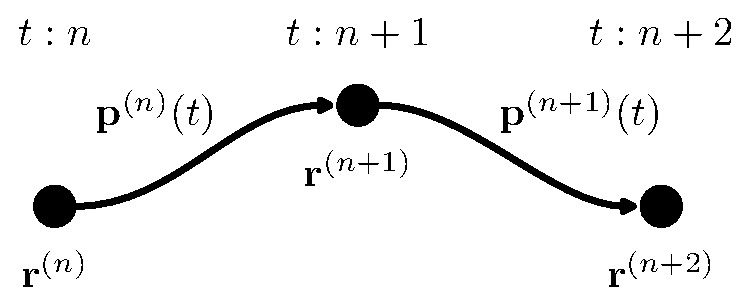
\includegraphics[width=0.35\textwidth]{boveda/Diagrama1.eps}
    \caption{Polynomials in the n-th position of cubic spline}
    \label{fig:3DSplinePoly}
\end{figure}

Given a set of $N$ points $\mathbf{r}^{(n)}\in\mathbb{R}^{3}$, $\forall$ $0\leq n \leq N-1$, 
we can generate a cubic spline with $N-2$ polynomials $\mathbf{p}^{(n)}(t)$, $\forall$ $0\leq n \leq N-2$, 
according to Fig. \ref{fig:3DSplinePoly}.
So that, it is fulfilled that 

\begin{equation}
\mathbf{p}^{(n)}(t)=
\begin{bmatrix}
x^{(n)}(t) & y^{(n)}(t) & z^{(n)}(t)
\end{bmatrix}^{T},
\end{equation}
where
\begin{equation}
x^{(n)}(t)=a_{x}^{(n)}+b_{x}^{(n)}(t-n)+c_{x}^{(n)}(t-n)^{2}+d_{x}^{(n)}(t-n)^{3},
\end{equation}
\begin{equation}
y^{(n)}(t)=a_{y}^{(n)}+b_{y}^{(n)}(t-n)+c_{y}^{(n)}(t-n)^{2}+d_{y}^{(n)}(t-n)^{3},
\end{equation}
\begin{equation}
z^{(n)}(t)=a_{z}^{(n)}+b_{z}^{(n)}(t-n)+c_{z}^{(n)}(t-n)^{2}+d_{z}^{(n)}(t-n)^{3}.
\end{equation}

%%%%%%%%%%%%%%%%%%%%%%%%%%%%%%%%%%%%%%%%%%%%%%%%%%%%%%%%%%%%%%%%%%%%%%%%%%%%%
\subsection{Matricial form of polynomials $\mathbf{p}^{(n)}(t)$}
For all values $0\leq n \leq N-2$, we know that
\begin{equation}
\mathbf{w}^{(n)}=
\left[
\begin{array}{cccc:cccc:cccc}
a_{x}^{(n)} & b_{x}^{(n)} & c_{x}^{(n)} & d_{x}^{(n)} & 
a_{y}^{(n)} & b_{y}^{(n)} & c_{y}^{(n)} & d_{y}^{(n)} & 
a_{z}^{(n)} & b_{z}^{(n)} & c_{z}^{(n)} & d_{z}^{(n)}
\end{array}
\right]^{T},
\end{equation}
\small
\begin{equation}\label{eq:Ant}
\mathbf{A}^{(n)}(t)=
\left[
\begin{array}{cccc:cccc:cccc}
1 & (t-n) & (t-n)^{2} & (t-n)^{3} &
0 & 0 & 0 & 0 &
0 & 0 & 0 & 0 \\
0 & 0 & 0 & 0 &
1 & (t-n) & (t-n)^{2} & (t-n)^{3} &
0 & 0 & 0 & 0 \\
0 & 0 & 0 & 0 &
0 & 0 & 0 & 0 &
1 & (t-n) & (t-n)^{2} & (t-n)^{3} 
\end{array}
\right],
\end{equation}
\normalsize

\begin{equation}\label{eq:primeder0}
\mathbf{p}^{(n)}(t)=
\mathbf{A}^{(n)}(t) \mathbf{w}^{(n)}.
\end{equation}

Additionally, we can define

\begin{equation}\label{eq:wvector}
\mathbf{w}
\equiv
\begin{bmatrix}
\mathbf{w}^{(0)}\\
\mathbf{w}^{(1)}\\
%\mathbf{w}^{(2)}\\
\vdots\\
\mathbf{w}^{(N-2)}\\
\end{bmatrix}
\in \mathbb{R}^{12(N-1)}
\end{equation}

%%%%%%%%%%%%%%%%%%%%%%%%%%%%%%%%%%%%%%%%%%%%%%%%%%%%%%%%%%%%%%%%%%%%%%%%%%%%%
\subsection{Derivative of $\mathbf{p}^{(n)}(t)$ with respect to escalar $t$}

\small
\begin{equation}\label{eq:primeder1}
\frac{\partial \mathbf{A}^{(n)}(t)}{\partial t}=
\left[
\begin{array}{cccc:cccc:cccc}
0 & 1 & 2(t-n) & 3(t-n)^{2} &
0 & 0 & 0 & 0 &
0 & 0 & 0 & 0 \\
0 & 0 & 0 & 0 &
0 & 1 & 2(t-n) & 3(t-n)^{2} &
0 & 0 & 0 & 0 \\
0 & 0 & 0 & 0 &
0 & 0 & 0 & 0 &
0 & 1 & 2(t-n) & 3(t-n)^{2} 
\end{array}
\right],
\end{equation}
\normalsize

\small
\begin{equation}\label{eq:primeder2}
\frac{\partial^{2} \mathbf{A}^{(n)}(t)}{\partial t^{2}}=
\left[
\begin{array}{cccc:cccc:cccc}
0 & 0 & 2 & 6(t-n) &
0 & 0 & 0 & 0 &
0 & 0 & 0 & 0 \\
0 & 0 & 0 & 0 &
0 & 0 & 2 & 6(t-n) &
0 & 0 & 0 & 0 \\
0 & 0 & 0 & 0 &
0 & 0 & 0 & 0 &
0 & 0 & 2 & 6(t-n) 
\end{array}
\right].
\end{equation}
\normalsize

 If we define 
 $\frac{\partial \mathbf{A}^{(n)}(t)}{\partial t} \equiv D_{t}\mathbf{A}^{(n)}(t)$
 and
 $\frac{\partial^{2} \mathbf{A}^{(n)}(t)}{\partial t^{2}} \equiv D_{t}^{2}\mathbf{A}^{(n)}(t)$, 
 then
 
\begin{align}\label{eq:primeder3a}
\frac{\partial \mathbf{p}^{(n)}(t)}{\partial t}
&=
D_{t}\mathbf{A}^{(n)}(t) \mathbf{w}^{(n)} \\
~
&=
\begin{bmatrix}
b_{x}^{(n)}+2(t-n) c_{x}^{(n)}+3(t-n)^{2} d_{x}^{(n)}\\
b_{y}^{(n)}+2(t-n) c_{y}^{(n)}+3(t-n)^{2} d_{y}^{(n)}\\
b_{z}^{(n)}+2(t-n) c_{z}^{(n)}+3(t-n)^{2} d_{z}^{(n)}
\end{bmatrix}
\end{align}


\begin{align}\label{eq:primeder3b}
\frac{\partial^{2} \mathbf{p}^{(n)}(t)}{\partial t^{2}}
&=
D_{t}^{2}\mathbf{A}^{(n)}(t) \mathbf{w}^{(n)}\\
~ 
&=
\begin{bmatrix}
2 c_{x}^{(n)}+6(t-n) d_{x}^{(n)}\\
2 c_{y}^{(n)}+6(t-n) d_{y}^{(n)}\\
2 c_{z}^{(n)}+6(t-n) d_{z}^{(n)}
\end{bmatrix}
\end{align}



%%%%%%%%%%%%%%%%%%%%%%%%%%%%%%%%%%%%%%%%%%%%%%%%%%%%%%%%%%%%%%%%%%%%%%%%%%%%%
%%%%%%%%%%%%%%%%%%%%%%%%%%%%%%%%%%%%%%%%%%%%%%%%%%%%%%%%%%%%%%%%%%%%%%%%%%%%%
\subsection{Conditions in 3D parametric cubic spline}\label{sec:boundarycubic}

%%%%%%%%%%%%%%%%%%%%%%%%%%%%%%%%%%%%%%%%%%%%%%%%%%%%%%%%%%%%%%%%%%%%%%%%%%%%%
\subsubsection{Boundary conditions in points}

Following the Fig. \ref{fig:3DSplinePoly}, 
we can affirm that for $0 \leq n\leq N-2$,
so that
\begin{equation}\label{eq:condition1}
\mathbf{p}^{(n)}(n)\approx \mathbf{r}^{(n)}
\in \mathbb{R}^{3},
\end{equation}

\begin{equation}\label{eq:condition2}
\mathbf{p}^{(N-2)}(N-1)\approx \mathbf{r}^{(N-1)}
\in \mathbb{R}^{3},
\end{equation}

\subsubsection{Matricial form of the boundary conditions in points}
Using 
the Eq. \ref{eq:primeder0} in 
the Eqs. \ref{eq:condition1} and \ref{eq:condition2},
we obtain for $0 \leq n\leq N-2$

\begin{equation}\label{eq:pointcond1}
\mathbf{A}^{(n)}(n) \mathbf{w}^{(n)}\approx \mathbf{r}^{(n)}
\in \mathbb{R}^{3},
\end{equation}

\begin{equation}\label{eq:pointcond2}
\mathbf{A}^{(N-2)}(N-1) \mathbf{w}^{(N-2)}\approx \mathbf{r}^{(N-1)}
\in \mathbb{R}^{3},
\end{equation}





where, using the Eq. \ref{eq:Ant}, we know that

\begin{equation}\label{eq:Q00}
\mathbf{A}^{(n)}(n+1)=
\left[
\begin{array}{cccc:cccc:cccc}
1 & 1 & 1 & 1 &
0 & 0 & 0 & 0 &
0 & 0 & 0 & 0 \\
0 & 0 & 0 & 0 &
1 & 1 & 1 & 1 &
0 & 0 & 0 & 0 \\
0 & 0 & 0 & 0 &
0 & 0 & 0 & 0 &
1 & 1 & 1 & 1 
\end{array}
\right]
\equiv \mathbf{Q}^{(0,0)}\in \mathbb{R}^{3\times 12},
\end{equation}

\begin{equation}\label{eq:Q01}
\mathbf{A}^{(n+1)}(n+1)
=
\mathbf{A}^{(n)}(n)
=
\left[
\begin{array}{cccc:cccc:cccc}
1 & 0 & 0 & 0 &
0 & 0 & 0 & 0 &
0 & 0 & 0 & 0 \\
0 & 0 & 0 & 0 &
1 & 0 & 0 & 0 &
0 & 0 & 0 & 0 \\
0 & 0 & 0 & 0 &
0 & 0 & 0 & 0 &
1 & 0 & 0 & 0 
\end{array}
\right]
\equiv \mathbf{Q}^{(0,1)}\in \mathbb{R}^{3\times 12},
\end{equation}

Thus,
using the Eqs. \ref{eq:Q00} and \ref{eq:Q01} in 
the Eqs. \ref{eq:pointcond1} and \ref{eq:pointcond2}, 
$\forall 0 \leq n\leq N-2$;
We can write the Eqs. \ref{eq:condition1} and \ref{eq:condition2} as 

\begin{equation}
\mathbf{P}
\mathbf{w}
\approx \mathbf{r}\in \mathbb{R}^{3N}.
\end{equation}

Where
\begin{equation}\label{eq:Pmat}
\mathbf{P}
\equiv
\begin{bmatrix}
\mathbf{Q}^{(0,1)} & \mathbf{0}         & \hdots & \mathbf{0} & \mathbf{0}         & \mathbf{0}\\
\mathbf{0}         & \mathbf{Q}^{(0,1)} & \hdots & \mathbf{0} & \mathbf{0}         & \mathbf{0}\\
\vdots             & \vdots             & \vdots & \vdots     & \vdots             & \vdots    \\ 
\mathbf{0}         & \mathbf{0}         & \hdots & \mathbf{0} & \mathbf{Q}^{(0,1)} & \mathbf{0}\\
\mathbf{0}         & \mathbf{0}         & \hdots & \mathbf{0} & \mathbf{0}         & \mathbf{Q}^{(0,1)}\\
\mathbf{0}         & \mathbf{0}         & \hdots & \mathbf{0} & \mathbf{0}         & \mathbf{Q}^{(0,0)}
\end{bmatrix}
\in \mathbb{R}^{3N\times 12(N-1)}
\end{equation}

and

\begin{equation}\label{eq:rvec}
\mathbf{r}
\equiv
\begin{bmatrix}
\mathbf{r}^{(0)}\\
\mathbf{r}^{(1)}\\
%\mathbf{w}^{(2)}\\
\vdots\\
\mathbf{r}^{(N-1)}\\
\end{bmatrix}
\in \mathbb{R}^{3N}
\end{equation}


%%%%%%%%%%%%%%%%%%%%%%%%%%%%%%%%%%%%%%%%%%%%%%%%%%%%%%%%%%%%%%%%%%%%%%%%%%%%%
\subsubsection{Continuity conditions in internal point}
Following the Fig. \ref{fig:3DSplinePoly}, 
we can affirm that for $0 \leq n\leq N-3$,
so that
\begin{equation}\label{eq:bound1}
\mathbf{p}^{(n)}(n+1)-\mathbf{p}^{n+1}(n+1)
\approx
\mathbf{0}\in \mathbb{R}^{3},
\end{equation}

\begin{equation}\label{eq:bound2}
\left.\frac{\partial\mathbf{p}^{(n)}(t)}{\partial t}\right|_{t=n+1}
-
\left.\frac{\partial\mathbf{p}^{n+1}(t)}{\partial t}\right|_{t=n+1}
\approx\mathbf{0}\in \mathbb{R}^{3},
\end{equation}

\begin{equation}\label{eq:bound3}
\left.\frac{\partial^{2}\mathbf{p}^{(n)}(t)}{\partial t^{2}}\right|_{t=n+1}
-
\left.\frac{\partial^{2}\mathbf{p}^{n+1}(t)}{\partial t^{2}}\right|_{t=n+1}
\approx\mathbf{0}\in \mathbb{R}^{3}.
\end{equation}

%%%%%%%%%%%%%%%%%%%%%%%%%%%%%%%%%%%%%%%%%%%%%%%%%%%%%%%%%%%%%%%%%%%%%%%%%%%%%
\subsubsection{Matricial form of the continuity conditions in internal point equation's}
Using % 
the Eqs. \ref{eq:primeder0}, \ref{eq:primeder1}, \ref{eq:primeder2}, \ref{eq:primeder3a} and \ref{eq:primeder3b} in 
the Eqs. \ref{eq:bound1}, \ref{eq:bound2} and \ref{eq:bound3},
we obtain for $0 \leq n\leq N-3$
\begin{equation}
 \mathbf{A}^{(n)}(n+1) \mathbf{w}^{(n)} - \mathbf{A}^{(n+1)}(n+1) \mathbf{w}^{(n+1)} 
 \approx
 \mathbf{0} \in \mathbb{R}^{3},
\end{equation}

\begin{equation}
D_{t}\mathbf{A}^{(n)}(n+1)
\mathbf{w}^{(n)}
-
D_{t}\mathbf{A}^{(n+1)}(n+1)
\mathbf{w}^{(n+1)}
\approx\mathbf{0}\in \mathbb{R}^{3},
\end{equation}


\begin{equation}
D_{t}^{2}\mathbf{A}^{(n)}(n+1)
\mathbf{w}^{(n)}
-
D_{t}^{2}\mathbf{A}^{(n+1)}(n+1)
\mathbf{w}^{(n+1)}
=\mathbf{0}\in \mathbb{R}^{3}.
\end{equation}

Grouping in a matrix

\begin{equation}
\begin{bmatrix}
\mathbf{A}^{(n)}(n+1) & -\mathbf{A}^{(n+1)}(n+1)\\
D_{t}\mathbf{A}^{(n)}(n+1) & -D_{t}\mathbf{A}^{(n+1)}(n+1)\\
D_{t}^{2}\mathbf{A}^{(n)}(n+1) & -D_{t}^{2}\mathbf{A}^{(n+1)}(n+1)
\end{bmatrix}
\begin{bmatrix}
\mathbf{w}^{(n)}\\
\mathbf{w}^{(n+1)}
\end{bmatrix}
\approx\mathbf{0}\in \mathbb{R}^{9},
\end{equation}


using the Eqs. \ref{eq:primeder1} and \ref{eq:primeder2}, 
we know that

\begin{equation}\label{eq:Q10}
D_{t} \mathbf{A}^{(n)}(n+1)
=
\left[
\begin{array}{cccc:cccc:cccc}
0 & 1 & 2 & 3 &
0 & 0 & 0 & 0 &
0 & 0 & 0 & 0 \\
0 & 0 & 0 & 0 &
0 & 1 & 2 & 3 &
0 & 0 & 0 & 0 \\
0 & 0 & 0 & 0 &
0 & 0 & 0 & 0 &
0 & 1 & 2 & 3 
\end{array}
\right]
\equiv \mathbf{Q}^{(1,0)}\in \mathbb{R}^{3\times 12},
\end{equation}

\begin{equation}\label{eq:Q11}
D_{t} \mathbf{A}^{(n+1)}(n+1)
=
\left[
\begin{array}{cccc:cccc:cccc}
0 & 1 & 0 & 0 &
0 & 0 & 0 & 0 &
0 & 0 & 0 & 0 \\
0 & 0 & 0 & 0 &
0 & 1 & 0 & 0 &
0 & 0 & 0 & 0 \\
0 & 0 & 0 & 0 &
0 & 0 & 0 & 0 &
0 & 1 & 0 & 0 
\end{array}
\right]
\equiv \mathbf{Q}^{(1,1)}\in \mathbb{R}^{3\times 12},
\end{equation}

\begin{equation}\label{eq:Q20}
D_{t}^{2} \mathbf{A}^{(n)}(n+1)
=
\left[
\begin{array}{cccc:cccc:cccc}
0 & 0 & 2 & 6 &
0 & 0 & 0 & 0 &
0 & 0 & 0 & 0 \\
0 & 0 & 0 & 0 &
0 & 0 & 2 & 6 &
0 & 0 & 0 & 0 \\
0 & 0 & 0 & 0 &
0 & 0 & 0 & 0 &
0 & 0 & 2 & 6 
\end{array}
\right]
\equiv \mathbf{Q}^{(2,0)}\in \mathbb{R}^{3\times 12},
\end{equation}

\begin{equation}\label{eq:Q21}
D_{t}^{2} \mathbf{A}^{(n+1)}(n+1)
=
\left[
\begin{array}{cccc:cccc:cccc}
0 & 0 & 2 & 0 &
0 & 0 & 0 & 0 &
0 & 0 & 0 & 0 \\
0 & 0 & 0 & 0 &
0 & 0 & 2 & 0 &
0 & 0 & 0 & 0 \\
0 & 0 & 0 & 0 &
0 & 0 & 0 & 0 &
0 & 0 & 2 & 0 
\end{array}
\right]
\equiv \mathbf{Q}^{(2,1)}\in \mathbb{R}^{3\times 12}.
\end{equation}

Thus,
using the Eqs. \ref{eq:Q00}, \ref{eq:Q01}, \ref{eq:Q10}, \ref{eq:Q11}, \ref{eq:Q20} and \ref{eq:Q21} in 
the Eqs. \ref{eq:bound1}, \ref{eq:bound2} and \ref{eq:bound3}, 
these can be rewritten for $0 \leq n\leq N-3$

\begin{equation}
\begin{bmatrix}
\mathbf{Q}^{(0,0)} & -\mathbf{Q}^{(0,1)}\\
\mathbf{Q}^{(1,0)} & -\mathbf{Q}^{(1,1)}\\
\mathbf{Q}^{(2,0)} & -\mathbf{Q}^{(2,1)}\\
\end{bmatrix}
\begin{bmatrix}
\mathbf{w}^{(n)}\\
\mathbf{w}^{(n+1)}
\end{bmatrix}
\approx\mathbf{0}\in \mathbb{R}^{9}
\end{equation}

Finally, 
concatenating to all values for $0 \leq n\leq N-3$
in the boundary conditions in internal point equation's, we obtain

\begin{equation}\label{eq:Qmat}
\mathbf{Q}
\equiv
\begin{bmatrix}
\mathbf{Q}^{(0,0)} & -\mathbf{Q}^{(0,1)} & \mathbf{0} & \mathbf{0} & \hdots & \mathbf{0} & \mathbf{0} & \mathbf{0}\\
\mathbf{Q}^{(1,0)} & -\mathbf{Q}^{(1,1)} & \mathbf{0} & \mathbf{0} & \hdots & \mathbf{0} & \mathbf{0} & \mathbf{0}\\
\mathbf{Q}^{(2,0)} & -\mathbf{Q}^{(2,1)} & \mathbf{0} & \mathbf{0} & \hdots & \mathbf{0} & \mathbf{0} & \mathbf{0}\\ \hdashline[2pt/2pt]
\mathbf{0} & \mathbf{Q}^{(0,0)} & -\mathbf{Q}^{(0,1)} & \mathbf{0} & \hdots & \mathbf{0} & \mathbf{0} & \mathbf{0}\\
\mathbf{0} & \mathbf{Q}^{(1,0)} & -\mathbf{Q}^{(1,1)} & \mathbf{0} & \hdots & \mathbf{0} & \mathbf{0} & \mathbf{0}\\
\mathbf{0} & \mathbf{Q}^{(2,0)} & -\mathbf{Q}^{(2,1)} & \mathbf{0} & \hdots & \mathbf{0} & \mathbf{0} & \mathbf{0}\\ \hdashline[2pt/2pt]
\vdots     & \vdots             & \vdots             & \vdots     & \vdots & \vdots     & \vdots     & \vdots    \\ \hdashline[2pt/2pt]
\mathbf{0} & \mathbf{0}         & \mathbf{0}         & \mathbf{0} & \hdots & \mathbf{0} & \mathbf{Q}^{(0,0)} & -\mathbf{Q}^{(0,1)}\\
\mathbf{0} & \mathbf{0}         & \mathbf{0}         & \mathbf{0} & \hdots & \mathbf{0} & \mathbf{Q}^{(1,0)} & -\mathbf{Q}^{(1,1)}\\
\mathbf{0} & \mathbf{0}         & \mathbf{0}         & \mathbf{0} & \hdots & \mathbf{0} & \mathbf{Q}^{(2,0)} & -\mathbf{Q}^{(2,1)}\\
\end{bmatrix}
\in \mathbb{R}^{9(N-2)\times 12(N-1)}
\end{equation}

\begin{equation}
\mathbf{Q}
\mathbf{w}
\approx\mathbf{0}\in \mathbb{R}^{9(N-2)}
\end{equation}


%%%%%%%%%%%%%%%%%%%%%%%%%%%%%%%%%%%%%%%%%%%%%%%%%%%%%%%%%%%%%%%%%%%%%%%%%%%%%
%%%%%%%%%%%%%%%%%%%%%%%%%%%%%%%%%%%%%%%%%%%%%%%%%%%%%%%%%%%%%%%%%%%%%%%%%%%%%

\subsection{Square curvature of a 3D parametric cubic spline}
\label{sec:curvaturemain}
We know by the Eq. (\ref{eq:curvaturekn}) that

\begin{equation}
\mathcal{K}_{(n)}(t)
=
\frac{\left\|{\mathbf{p}^{(n)}}'(t) \times {\mathbf{p}^{(n)}}''(t) \right\|}
{\left\|{\mathbf{p}^{(n)}}'(t)\right\|^{3}}
\end{equation}

If we calculate the square curvature $\mathcal{K}_{(n)}^{2}(t)$ for the boundary cases of the curve $\mathbf{p}^{(n)}(t)$, 
when $t\equiv n$ and $t\equiv n+1$,
then we obtain $\mathcal{K}_{(n)}^{2}(n)$ and $\mathcal{K}_{(n)}^{2}(n+1)$, respectively
\begin{equation}\label{eq:curvature:K2nn}
\mathcal{K}_{(n)}^{2}(n)
=
\frac{\left\|
\left( \mathbf{Q}^{(1,1)} \mathbf{w}^{(n)} \right)
\times 
\left( \mathbf{Q}^{(2,1)} \mathbf{w}^{(n)} \right)
\right\|^{2}}
{\left\| \mathbf{Q}^{(1,1)} \mathbf{w}^{(n)} \right\|^{6}}
\end{equation}

\begin{equation}\label{eq:curvature:K2nn1}
\mathcal{K}_{(n)}^{2}(n+1)
=
\frac{\left\|
\left( \mathbf{Q}^{(1,0)} \mathbf{w}^{(n)} \right)
\times 
\left( \mathbf{Q}^{(2,0)} \mathbf{w}^{(n)} \right)
\right\|^{2}}
{\left\| \mathbf{Q}^{(1,0)} \mathbf{w}^{(n)} \right\|^{6}}
\end{equation}


If we use the Eq. (\ref{eq:cuvaturepartial}) to differentiate the Eqs. (\ref{eq:curvature:K2nn}) and (\ref{eq:curvature:K2nn1})
with respect to $\mathbf{w}^{(n)}$, 
we obtain the Eqs. (\ref{eq:curvature:der:K2nn}) and (\ref{eq:curvature:der:K2nn1}), respectively.

\begin{equation}\label{eq:curvature:der:K2nn}
\begin{split}
\frac{
\partial 
\mathcal{K}_{(n)}^{2}(n)
}
{
\partial \mathbf{w}^{(n)}
}
& = 
2
\frac{
\left\|{\mathbf{p}^{(n)}}''(n)\right\|^2
\mathbf{Q}^{(1,1)T} {\mathbf{p}^{(n)}}'(n)
+
\left\|{\mathbf{p}^{(n)}}'(n)\right\|^2
\mathbf{Q}^{(2,1)T} {\mathbf{p}^{(n)}}''(n)
}
{\left\| {\mathbf{p}^{(n)}}'(n) \right\|^{6}}\\[10pt]
& - 
2
\frac
{
\left(
{{\mathbf{p}^{(n)}}'(n)}^{T}
{\mathbf{p}^{(n)}}''(n)
\right)
\left(
\mathbf{Q}^{(1,1)T}{\mathbf{p}^{(n)}}''(n)
+
\mathbf{Q}^{(2,1)T}{\mathbf{p}^{(n)}}'(n)
\right)
}
{\left\| {\mathbf{p}^{(n)}}'(n) \right\|^{6}}\\[10pt]
& - 
6
\frac
{
\mathcal{K}_{(n)}^{2}(n)
\mathbf{Q}^{(1,1)T}{\mathbf{p}^{(n)}}'(n)
}
{\left\| {\mathbf{p}^{(n)}}'(n) \right\|^{2}}
\end{split}
\end{equation}

and

\begin{equation}\label{eq:curvature:der:K2nn1}
\begin{split}
\frac{
\partial 
\mathcal{K}_{(n)}^{2}(n+1)
}
{
\partial \mathbf{w}^{(n)}
}
& = 
2
\frac{
\left\|{\mathbf{p}^{(n)}}''(n+1)\right\|^2
\mathbf{Q}^{(1,0)T} {\mathbf{p}^{(n)}}'(n+1)
+
\left\|{\mathbf{p}^{(n)}}'(n+1)\right\|^2
\mathbf{Q}^{(2,0)T} {\mathbf{p}^{(n)}}''(n+1)
}
{\left\| {\mathbf{p}^{(n)}}'(n+1) \right\|^{6}}\\[10pt]
& - 
2
\frac
{
\left(
{{\mathbf{p}^{(n)}}'(n+1)}^{T}
{\mathbf{p}^{(n)}}''(n+1)
\right)
\left(
\mathbf{Q}^{(1,0)T}{\mathbf{p}^{(n)}}''(n+1)
+
\mathbf{Q}^{(2,0)T}{\mathbf{p}^{(n)}}'(n+1)
\right)
}
{\left\| {\mathbf{p}^{(n)}}'(n+1) \right\|^{6}}\\[10pt]
& - 
6
\frac
{
\mathcal{K}_{(n)}^{2}(n+1)
\mathbf{Q}^{(1,0)T}{\mathbf{p}^{(n)}}'(n+1)
}
{\left\| {\mathbf{p}^{(n)}}'(n+1) \right\|^{2}}
\end{split}
\end{equation}

\begin{comment}
Finally

\begin{equation}
\frac{
\partial 
\mathcal{K}_{(n)}^{2}(n+1)
}
{
\partial \mathbf{w}^{(n)}
}
\end{equation}
\end{comment}

%%%%%%%%%%%%%%%%%%%%%%%%%%%%%%%%%%%%%%%%%%%%%%%%%%%%%%%%%%%%%%%%%%%%%%%%%%%%%
%%%%%%%%%%%%%%%%%%%%%%%%%%%%%%%%%%%%%%%%%%%%%%%%%%%%%%%%%%%%%%%%%%%%%%%%%%%%%
\subsection{Cost function in 3D parametric cubic spline}

%%%%%%%%%%%%%%%%%%%%%%%%%%%%%%%%%%%%%%%%%%%%%%%%%%%%%%%%%%%%%%%%%%%%%%%%%%%%%
\subsubsection{Cost function of fitting the cubic spline in the points $\mathbf{r}^{(n)}$}

Following the explanation in the Section \ref{sec:boundarycubic},
the equation that should be fulfilled to fit the cubic spline in the points can be represented in the next equation

\begin{equation}
\begin{bmatrix}
\mathbf{P}\\
\mathbf{Q}
\end{bmatrix}
\mathbf{w}
\approx
\begin{bmatrix}
\mathbf{r}\\
\mathbf{0}
\end{bmatrix}
\in \mathbb{R}^{12(N-1)-6}
\end{equation}

Defining the cost function $E_{1}(\mathbf{w})$ of fitting of cubic spline in the points $\mathbf{r}^{(n)}$,
$\forall 0\leq n\leq N-1$

\begin{equation}\label{eq:costfunc1}
E_{1}(\mathbf{w})
=
\left\|
\begin{bmatrix}
\mathbf{P}\\
\mathbf{Q}
\end{bmatrix}
\mathbf{w}
-
\begin{bmatrix}
\mathbf{r}\\
\mathbf{0}
\end{bmatrix}
\right\|_{\mathbf{D}}^{2}
\end{equation}
where $\mathbf{D}\in \mathbb{R}^{(12N-18)\times(12N-18)}$ is a diagonal matrix with the weight of each line equation
and $\left\|\mathbf{a}\right\|_{\mathbf{D}}^{2}\equiv \mathbf{a}^{T}\mathbf{D}\mathbf{a}$.


Applying the derivative in relation to vector $\mathbf{w}$
\cite[pp. 11]{petersen2008matrix}
in the cost function $E_{1}(\mathbf{w})$ of Eq. \ref{eq:costfunc1}, 
we obtain

\begin{equation}\label{eq:DE1}
\frac{\partial E_{1}(\mathbf{w})}{\partial \mathbf{w}}
=
2
\begin{bmatrix}
\mathbf{P}\\
\mathbf{Q}
\end{bmatrix}^{T}
\mathbf{D}
\left(
\begin{bmatrix}
\mathbf{P}\\
\mathbf{Q}
\end{bmatrix}
\mathbf{w}
-
\begin{bmatrix}
\mathbf{r}\\
\mathbf{0}
\end{bmatrix}
\right)
\end{equation}

%%%%%%%%%%%%%%%%%%%%%%%%%%%%%%%%%%%%%%%%%%%%%%%%%%%%%%%%%%%%%%%%%%%%%%%%%%%%%
\subsubsection{Cost function of curvature the cubic spline in the points $\mathbf{r}^{(n)}$}

Following the explanation in the Section \ref{sec:curvaturemain},
the equation relative to the curvature that should be minimized can be represented in the next equation




\begin{equation}
E_{2}
=
\frac{1}{2(N-1)}
\sum\limits_{n=0}^{N-2}
\left\{
\mathcal{K}_{(n)}^{2}(n)
+
\mathcal{K}_{(n)}^{2}(n+1)
\right\}.
\end{equation}

Derivating in function of $\mathbf{w}$

\begin{equation}
\frac{\partial E_{2}}{\partial \mathbf{w}^{(n)}}
=
\frac{1}{2(N-1)}
\left\{
\frac{
\partial 
\mathcal{K}_{(n)}^{2}(n)
}{\partial \mathbf{w}^{(n)}}
+
\frac{
\partial 
\mathcal{K}_{(n)}^{2}(n+1)
}{\partial \mathbf{w}^{(n)}}
\right\}
\end{equation}

\begin{equation}\label{eq:DE2}
\frac{\partial E_{2}}{\partial \mathbf{w}}
=
\begin{bmatrix}
\frac{\partial E_{2}}{\partial \mathbf{w}^{(0)}}\\[4pt]
\frac{\partial E_{2}}{\partial \mathbf{w}^{(1)}}\\[4pt]
\vdots\\[4pt]
\frac{\partial E_{2}}{\partial \mathbf{w}^{(N-2)}}
\end{bmatrix}
=
\frac{1}{2(N-1)}
\begin{bmatrix}
%
\frac{
\partial 
\mathcal{K}_{(0)}^{2}(0)
}{\partial \mathbf{w}^{(0)}}
+
\frac{
\partial 
\mathcal{K}_{(0)}^{2}(1)
}{\partial \mathbf{w}^{(0)}}\\[4pt]
%
\frac{
\partial 
\mathcal{K}_{(1)}^{2}(1)
}{\partial \mathbf{w}^{(1)}}
+
\frac{
\partial 
\mathcal{K}_{(1)}^{2}(2)
}{\partial \mathbf{w}^{(1)}}\\[4pt]
%
\vdots\\[4pt]
\frac{
\partial 
\mathcal{K}_{(N-2)}^{2}(N-2)
}{\partial \mathbf{w}^{(N-2)}}
+
\frac{
\partial 
\mathcal{K}_{(N-2)}^{2}(N-1)
}{\partial \mathbf{w}^{(N-2)}}\\
%
\end{bmatrix}
.
\end{equation}

%%%%%%%%%%%%%%%%%%%%%%%%%%%%%%%%%%%%%%%%%%%%%%%%%%%%%%%%%%%%%%%%%%%%%%%%%%%%%
\subsubsection{Total cost function of 3D parametric cubic spline}
\label{sec:TotalCostFunc}

Defining the total cost function $E(\mathbf{w})$ as

\begin{equation}
E(\mathbf{w})=E_{1}(\mathbf{w})+\beta E_{2}(\mathbf{w})
\end{equation}

\begin{equation}
E(\mathbf{w})
=
\left\|
\begin{bmatrix}
\mathbf{P}\\
\mathbf{Q}
\end{bmatrix}
\mathbf{w}
-
\begin{bmatrix}
\mathbf{r}\\
\mathbf{0}
\end{bmatrix}
\right\|_{\mathbf{D}}^{2}
+\beta 
\left[
\frac{1}{2(N-1)}
\sum\limits_{n=0}^{N-2}
\left\{
\mathcal{K}_{(n)}^{2}(n)
+
\mathcal{K}_{(n)}^{2}(n+1)
\right\}
\right].
\end{equation}

where 
\begin{itemize}
\item the constant matrix $\mathbf{P}$ is defined in Eq. (\ref{eq:Pmat}),
\item the constant matrix $\mathbf{Q}$ is defined in Eq. (\ref{eq:Qmat}),
\item the diagonal matrix $\mathbf{D}$ contains hyperparameters that assign weights to boundary and continuity conditions,
\item the constant vector $\mathbf{r}$ is an input position data described in Eq. (\ref{eq:rvec}),
\item the vector $\mathbf{w}$ has the parameters of spline as described in Eq. (\ref{eq:wvector}),
\item the scalar $\beta$ serves as a hyperparameter to balance the significance of $E_{2}(\mathbf{w})$ relative to $E_{1}(\mathbf{w})$,
\item the scalar $\mathcal{K}_{(n)}^{2}(n)$ is determined using Eq. (\ref{eq:curvature:K2nn}) and 
\item the scalar $\mathcal{K}_{(n)}^{2}(n+1)$ is determined using Eq. (\ref{eq:curvature:K2nn1}).
\end{itemize}
%%%%%%%%%%%%%%%%%%%%%%%%%%%%%%%%%%%%%%%%%%%%%%%%%%%%%%%%%%%%%%%%%%%%%%%%%%%%%
\subsection{Parameter calculus of 3D parametric cubic spline}
\label{sec:solvecubicspline}
Using the gradient descent technique, we obtain

\begin{equation}
\mathbf{w}_{i+1}
\leftarrow 
\mathbf{w}_{i}
-
\alpha
\left.
\frac{\partial 
\left\{
E_{1}(\mathbf{w})+\beta E_{2}(\mathbf{w})
\right\}
}{\partial \mathbf{w}}
\right|_{\mathbf{w}=\mathbf{w}_{i}}.
\end{equation}

Applying the Eqs. \ref{eq:DE1}, \ref{eq:DE2} we obtain

\begin{equation}
\mathbf{w}_{i+1}
\leftarrow 
\mathbf{w}_{i}
-
\alpha
\left\{
\left.
\frac{\partial E_{1}(\mathbf{w})}{\partial \mathbf{w}}
\right|_{\mathbf{w}=\mathbf{w}_{i}}
+
\beta
\left.
\frac{\partial E_{2}(\mathbf{w})}{\partial \mathbf{w}}
\right|_{\mathbf{w}=\mathbf{w}_{i}}
\right\}
\end{equation}

\begin{equation}
\mathbf{w}_{i+1}
\leftarrow 
\mathbf{w}_{i}
-
\alpha
\left\{
2
\begin{bmatrix}
\mathbf{P}\\
\mathbf{Q}
\end{bmatrix}^{T}
\mathbf{D}
\left(
\begin{bmatrix}
\mathbf{P}\\
\mathbf{Q}
\end{bmatrix}
\mathbf{w}_{i}
-
\begin{bmatrix}
\mathbf{r}\\
\mathbf{0}
\end{bmatrix}
\right)
+
\frac{\beta}{2(N-1)}
\begin{bmatrix}
%
\frac{
\partial 
\mathcal{K}_{(0)}^{2}(0)
}{\partial \mathbf{w}^{(0)}}
+
\frac{
\partial 
\mathcal{K}_{(0)}^{2}(1)
}{\partial \mathbf{w}^{(0)}}\\[4pt]
%
\frac{
\partial 
\mathcal{K}_{(1)}^{2}(1)
}{\partial \mathbf{w}^{(1)}}
+
\frac{
\partial 
\mathcal{K}_{(1)}^{2}(2)
}{\partial \mathbf{w}^{(1)}}\\[4pt]
%
\vdots\\[4pt]
\frac{
\partial 
\mathcal{K}_{(N-2)}^{2}(N-2)
}{\partial \mathbf{w}^{(N-2)}}
+
\frac{
\partial 
\mathcal{K}_{(N-2)}^{2}(N-1)
}{\partial \mathbf{w}^{(N-2)}}\\
%
\end{bmatrix}
\right\}
\end{equation}

where $\alpha$ and $\beta$ are learning hyper-parameters and 
$\mathbf{w}_{0}$ can be a random vector or can
be calculated following a 3D parametric linear spline,
see Section \ref{sec:solvelinearspline}.
The iteration follows until a maximum number of iterations $i$ or until it reaches a
minimum defined error $E_1(\mathbf{w}_{i})$. 




\printbibliography

\end{document}
